\documentclass[12pt, a4paper]{article}

\usepackage{tikz}
\usepackage{setspace}


\begin{document}
\begin{titlepage}
    \centering
    {\scshape\Huge Software Architecture \par}
    \vspace{1cm}
    
\includegraphics[width=0.7\textwidth]{team-logo}\par\vspace{1cm}
    {\scshape\huge OpenID Connect Doctor \par}
    {\scshape\Large Project 8 \par}
\end{titlepage}
\onehalfspacing
\section{Runtime Components}
\begin{figure}[!h]
    \centering
    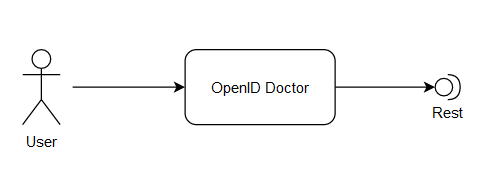
\includegraphics[width=.7\textwidth]{runtime_comp}
\end{figure}

\noindent {The OpenID Connect Doctor is a standalone CLI tool, that should be able to run on as many Operating Systems as possible. Furthermore, the application is required to work without the user having to install any additional programs. For this reason, it was decided, that the OpenID Connect Doctor should consist of only a single NodeJS application and use as few dependencies as possible. As the OpenID Connect Doctor must request tokens from an authorization server using OpenID Connect, it requires an interface to connect to a given authorization server using REST. To fully fulfill its task, the OpenID Connect Doctor is split into multiple smaller internal components, which carry out different tasks like requesting a token, decoding a token, etc. }

\newpage
\section{Code Components}
\begin{figure}[!h]
    \centering
    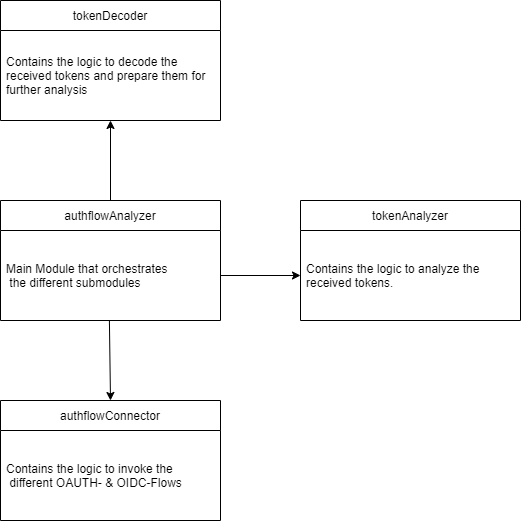
\includegraphics[width=\textwidth]{Code-Components}
\end{figure}

\noindent The code of the application will consist of multiple smaller classes, that each are responsible for a certain part of the application:
\begin{description}
\item[authflowConnector]: This class will contain the logic to send HTTP-requests to the different Identity-Providers and process the returned HTTP-response (e.g. for the different OIDC-Login-Flows).
\item[tokenDecoder]: This class will contain the logic to decode and transform the received access and id-tokens into a format that can be analyzed by the rest of the application.
\item[tokenAnalyzer]: This class will contain the logic to analyze the prepared information and report these information to the user (e.g. via the terminal or a logfile)
\item[authflowAnalyzer]: This class will reference the other three class and will be responsible for orchestrating the different functions. Additionally it will also include input-validation, global error-handling and configuration.
\end{description}
The reason for this split is to keep a certain level of separation between the different parts of the software, so it is easier to modify and test them.

\section{Technology Stack}
%\begin{center}
%\begin{tabular}{|p{1.5cm}|p{9cm}|p{1.5cm}|p{2cm}|}
%\hline
%\textbf{Type} & Programming Language & & \\
%\hline
%\textbf{Name} & \textbf{Description} & \textbf{Version} & \textbf{License}\\
%\hline
%NodeJS & Programming Language used to implement the application & 16.15.0 & MIT License\\
%\hline
%\end{tabular}\vspace{1cm}

%\begin{tabular}{|p{1.5cm}|p{9cm}|p{1.5cm}|p{2cm}|}
%    \hline
%    \textbf{Type} & Package Manager & & \\
%    \hline
%    \textbf{Name} & \textbf{Description} & \textbf{Version} & \textbf{License}\\
%    \hline
%    npm\textcolor{white}{aaa} & Package Manager is used in combination with the Programming Language to potentionally add additional libraries to create the application & 8.5.5 & Artistic License 2.0\\
%    \hline
%\end{tabular}\vspace{1cm}

%\begin{tabular}{|p{1.5cm}|p{9cm}|p{1.5cm}|p{2cm}|}
%\hline
%\textbf{Type} & Frameworks & & \\
%\hline
%\textbf{Name} & \textbf{Description} & \textbf{Version} & \textbf{License}\\
%\hline
%NestJS & Fullstack Development Framework for efficient, scalable Node.js server-side %applications & 8.4.4 & MIT License\\
%\hline
%Fastify & Node.js Framework to receive fast real-time applications running in NestJS intead of Express & 4.0.0 & MIT License\\
%\hline
%\end{tabular}\vspace{1cm}


%\begin{tabular}{|p{1.5cm}|p{9cm}|p{1.5cm}|p{2cm}|}
%    \hline
%    \textbf{Type} & Version Control & & \\
%    \hline
%    \textbf{Name} & \textbf{Description} & \textbf{Version} & \textbf{License}\\
%    \hline
%    Git\textcolor{white}{aaaaa} & Version Control employed to syoncronize to code with the developers  & - & GPL-2.0-only\\
%    \hline
%\end{tabular}
 
%\end{center}
\subsection*{NodeJS}


In our project we are using Node Js as our programming language. Node.js is an open-source, cross-platform, back-end JavaScript runtime environment that runs on the V8 engine and executes JavaScript code outside a web browser.Node.js represents a "JavaScript everywhere" paradigm,[6] unifying web-application development around a single programming language, rather than different languages for server-side and client-side scripts.

\begin{itemize}
    \item License: MIT License
    \item Operating system: z/OS, Linux, macOS, Microsoft Windows, SmartOS, FreeBSD, OpenBSD, IBM AIX
    \item Type: Runtime environment
    \item Version: 16.15.0
\end{itemize}


\subsection*{NestJS}



We have chosen NestJS because it has got additional features and libraries integrated for authentication. It is usable via cli and it is also possible to create frontends with it. Our application should be also applicable in real-time in the best case. 

\begin{itemize}
    \item License: MIT License
    \item Operating system: z/OS, Linux, macOS, Microsoft Windows, SmartOS, FreeBSD, OpenBSD, IBM AIX
    \item Type: Fullstack Development Framework for efficient, scalable Node.js server-side 
    \item Version: 8.4.4
\end{itemize}

\subsection*{Fastify}

NestJS is configured based on the framework Express as a default, but it is compatible with Fastify. Fastify can integrate the speed for real-time applications into NestJS, that the user does not have to wait for the response such a long time. 
NestJS and Fastify are both well maintained nodejs frameworks, which are also used for Enterprise open-source applications. Additionally, there is also a lot of documentation available, how to use it (incl. books).

\begin{itemize}
    \item License: MIT License
    \item Operating system:  Linux, macOS, Microsoft Windows
    \item Type: Node.js Framework to receive fast real-time applications running in NestJS intead of Express
    \item Version: 4.0.0
\end{itemize}

\subsection*{NPM}

With Node Js as programming language, we are using npm is a package manager.It's a JavaScript programming language maintained by npm, Inc. npm is the default package manager for the JavaScript runtime environment Node.js. npm can manage packages that are local dependencies of a particular project, as well as globally-installed JavaScript tools.

\begin{itemize}
    \item License: Artistic License 2.
    \item Platform: Cross-platform
    \item Type: Package manager
    \item Version: 8.5.5
\end{itemize}

\subsection*{GIT}

For the version control, we are using git in our project. Git is a software for tracking changes in any set of files, usually used for coordinating work among programmers collaboratively developing source code during software development.

\begin{itemize}
    \item License: GPL-2.0-only
    \item Operating system: POSIX (Linux, macOS, Solaris, AIX), Windows
    \item Type: Version contro
    \item Version: 2.36.1
\end{itemize}

\noindent The customer has suggested nodejs as the preferred language, because it has been used very much in their own technology stack. nodejs 16 is an LTS version with long-term support. Additionally it is available for Windows and openSUSE Tumbleweed (Linux). That is the reason for this suggestion, that the software can be developed based on multiple operating systems. \\
The package manager npm 8.5.5 is integrated into nodejs 16. Therefore, we are using this version.


\end{document}